\vspace{-5mm}
\section{Introduction}
\label{sec:intro}

\begin{figure*}[t]
    \centering
    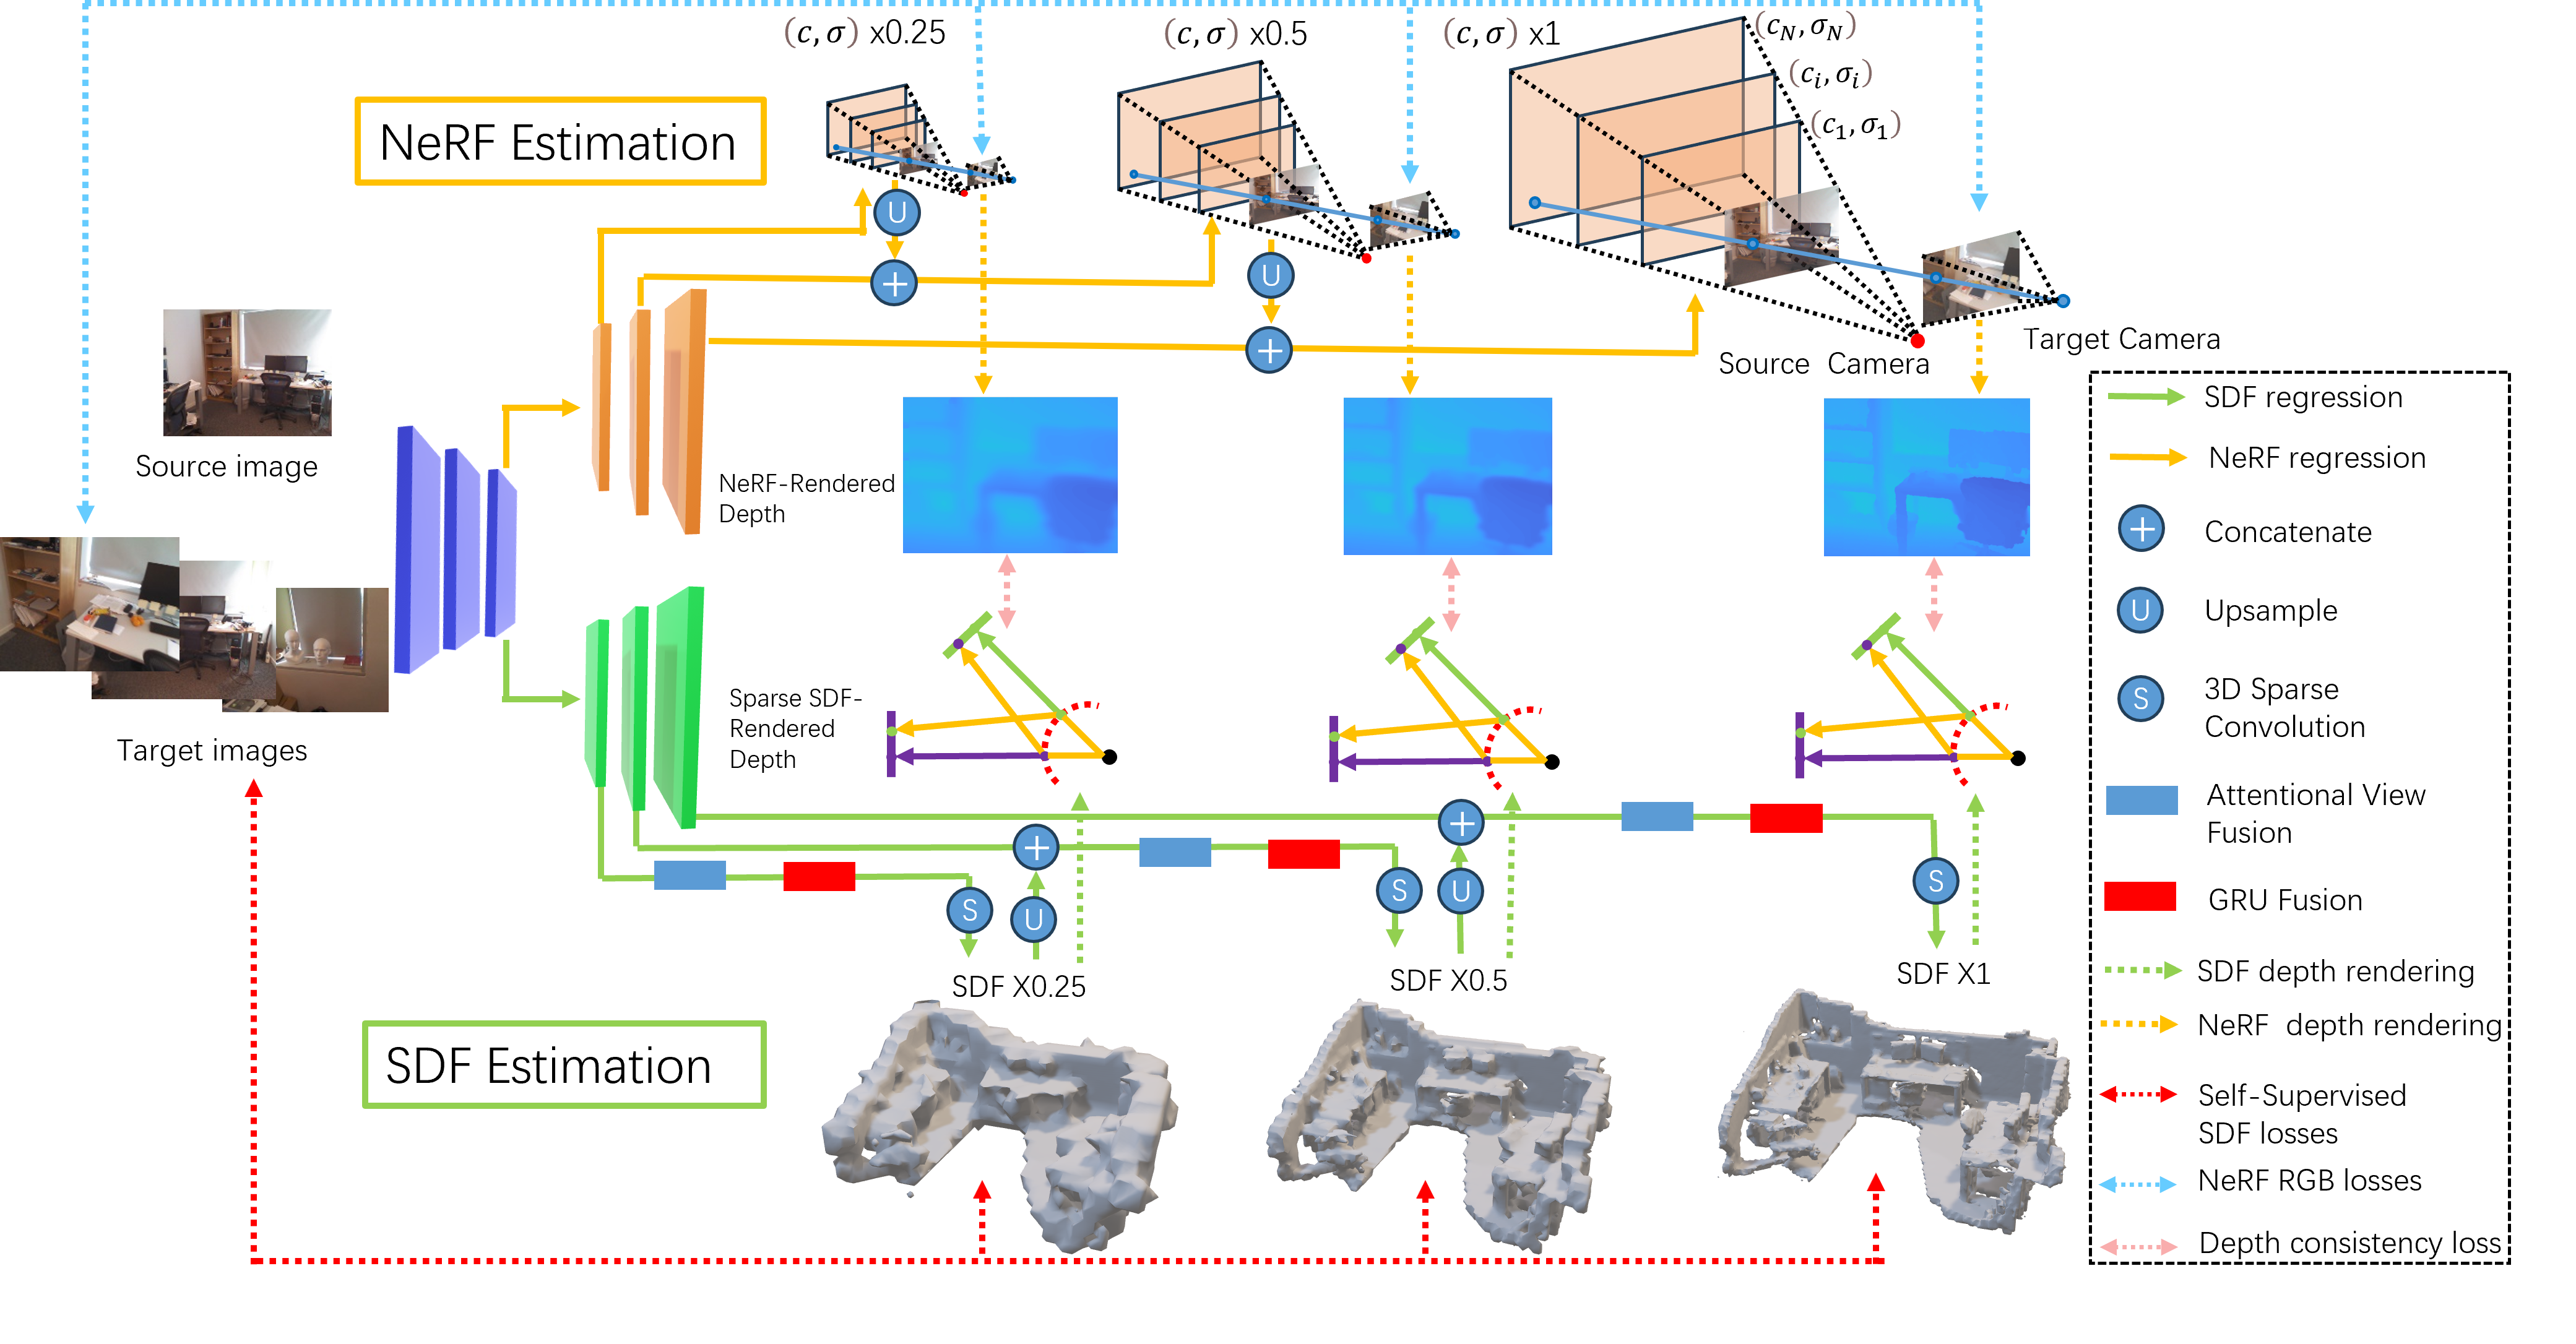
\includegraphics[width=\linewidth]{figures/pipeline.png}
    \vspace{-12mm}
    \caption{\textbf{MonoSelfRecon Pipeline.} We use monocular RGB sequence to estimate explicit 3D mesh of generalizble indoor scenes under purely self-supervision free of SDF or depth annotations. A coarse-to-fine architecture is used for both SDF and NeRF decoders, where our proposed self-supervised losses are used between SDF-inputRGB, NeRF-inputRGB, and SDF-NeRF.}
    \label{fig:pipeline}
    \vspace{-5mm}
\end{figure*}


\quad 3D scene reconstruction is one of the most important problems in 3D computer vision, robotics, virtual reality, autonomous driving and so on. Indoor 3DR is even more challenging because of the large texture-less region and complicated relations between objects. As more complicated and accurate models emerge, the main concern shifts to three standards: 1. Self-supervised training without laborious large-amount of annotations in depth or SDF, 2. Generalizable to same type of scenes, and 3. Explicit 3D mesh representations.

\begin{table}[]
\setlength\tabcolsep{1pt}
\footnotesize
\begin{tabular}{l|c|c|c}
\hline
\diagbox{Methods}{Standards}             & \multicolumn{1}{l|}{Self-Supervised} & \multicolumn{1}{l|}{Generalizable} & \multicolumn{1}{l}{Explicit 3D Mesh} \\ \hline
Self-supervised Depth & \textbf{\checkmark} & \textbf{\checkmark} & \ding{55} \\
Supervised Depth      & \ding{55} & \textbf{\checkmark}  & \ding{55}    \\
Supervised Voxel-SDF  & \ding{55} & \textbf{\checkmark}  & \textbf{\checkmark}    \\
Implicit NeRF         & \textbf{\checkmark}  & \ding{55} & \ding{55}          \\
Explicit SDF-NeRF     & \textbf{\checkmark}  & \ding{55} & \textbf{\checkmark}   \\ \hline
\textbf{Ours}  & \textbf{\checkmark}  & \textbf{\checkmark} & \textbf{\checkmark}  \\ \hline
\end{tabular}
\vspace{-3mm}
\caption{\textbf{Monocular 3DR measured in three major standards.}}
\label{table:3dr class}
\vspace{-7mm}
\end{table}


Explicit monocular 3DR models originate from depth estimation \cite{kineticfusion, 3dgo, vif, mvdepthnet, smartphone, neuralrgb, mvstempo}, where depth maps can be directly supervised with pixel-wise depth ground truth. Depth maps can be also self-supervised by continuous RGB sequences from multiple camera views, with or without camera poses. Under constraints such as temporal smoothness, multiple key frames are selected from continuous depth map sequence, fused to global 3D volume and integrate ``Truncated Signed Distance Function" value (TSDF) \cite{kineticfusion} for each voxel within the truncation distance. 3D surface mesh can be obtained from ``marching cube'' algorithm with estimated TSDF \cite{marchingcube}. However, because of the depth inconsistency in multi-views, directly fusing depth estimation for TSDF may cause it either layered or too sparse. Additionally, using depth maps from multiple views for TSDF fusion typically causes large overlapping regions, which is a waste of computation in inference\cite{neucon}. Later works \cite{atlas, neucon, vortx} overcome the limitations by pre-defining 3D voxels and directly regressing SDF for each voxel. However, these works must be trained in supervision with laboriously large amount of fine-grained SDF annotations fusing from depth map ground truth.

Implicit monocular 3DR works start to dominate with the emergence of NeRF\cite{nerf}. One advantage of implicit 3DR over explicit ones is its purely self-supervised training. With RGB sequence from different camera poses, NeRF reconstructs scenes in implicit representation by synthesizing images from new views. Recently, State-of-the-art (SOTA) works introduce implicit SDF function to NeRF, where the SDF-NeRF can estimate explicit SDF values w.r.t any specified 3D position in the scene \cite{hnerf, isdf, manhattansdf, monosdf, volsdf, neuris}. However, these 3DR works are still non-generalizable to other scenes. Although few works such as \cite{pixelnerf,mpi-nerf} make NeRF generalizable, the generalization has not been extended to estimate explicit SDF values.

We summarize current 3DR methods based on the three standards in Table \ref{table:3dr class}, where each type of the method is discussed in section \ref{sec:related_works}. Different to all existing works, where the 3DR either requires large amount of annotated ground truth, or non-generalizable, or not explicit in 3D representation, our work overcomes these three concerns altogether. Our key contributions are:

\begin{itemize}[leftmargin=0.2cm]
\setlength{\itemsep}{0pt}
\setlength{\parsep}{0pt}
\setlength{\parskip}{0pt}

\item We propose a novel framework ``MonoSelfRecon'' that first time achieves \textbf{explicit 3D mesh} reconstruction for
\textbf{generalizable} indoor scenes with monocular RGB sequence by purely \textbf{self-supervised} training on voxel-SDF, which is different to all existing works.

\item We propose novel self-supervised losses and conduct purely self-supervised training without SDF or depth ground truth. Experiments show that our approach outperforms the best self-supervised generalizable indoor 3DR (depth-based) works, and is comparable to fully-supervised works.

\item Our proposed self-supervised losses can be used together with supervised losses to boost fully supervised training. The framework is not limited to specific models but free to extend to any models with voxel-SDF estimation. Consequently, it keeps the advantages of the original model, such as inference speed and meomory efficiency.

\end{itemize}
